\documentclass[12pt]{book}
\usepackage[plainpages=false,hypertexnames=TRUE]{hyperref}

%
% Farbige Tabelleneinträge
\usepackage[table,xcdraw]{xcolor}
\usepackage{longtable}

% Globale Dokumentendefinitionen.
\newcommand{\bhtAuthor}{Wilfried Pahl}
\newcommand{\bhtTitle}{Evaluierung und Optimierung von Large Language Models für die Entwicklung von Webanwendungen}
\newcommand{\bhtSubtitle}{Ein Ansatz zur Verbesserung des Entwicklungsprozesses bei Softwareprojekten}
\newcommand{\bhtDocumentType}{Masterthesis\\für den Master of Science Studiengang Medieninformatik}
\newcommand{\bhtMatriculationNumber}{901932}
\newcommand{\bhtCourse}{Online Medieninformatik}
\newcommand{\bhtTown}{Temmen-Ringenwalde}

\newcommand{\bhtUniversity}{Berliner Hochschule für Technik}
\newcommand{\bhtCaretakerFirst}{Prof. Dr. S. Edlich}
\newcommand{\bhtCaretakerUniversityFirst}{Berliner Hochschule für Technik}


\newcommand{\bookThesisType}{Masterarbeit}
\newcommand{\bookTitle}{Evaluierung und Optimierung von Large Language Models für die Entwicklung von Webanwendungen}
\newcommand{\bookSubTitle}{Ein Ansatz zur Verbesserung des Entwicklungsprozesses bei Softwareprojekten}

% Globale Farbdefinition.
\usepackage{xcolor}
% Colors by SV Group
% \definecolor{BhtPrimaryColor}{HTML}{690D23}
% \definecolor{BhtGrey}{HTML}{000000}

% Colors by BHT
\definecolor{BhtColorAnthrazit}{HTML}{555555}
\definecolor{BhtColorRed}{HTML}{EA3B07}
\definecolor{BhtColorYellow}{HTML}{FFC900}
\definecolor{BhtColorPetrol}{HTML}{00A0AA}
\definecolor{BhtColorBlue}{HTML}{004282}

\definecolor{BhtPrimaryColor}{HTML}{004282} % Blau
\definecolor{BhtGrey}{HTML}{555555}

%--------------------------------------------------------
% Deutsch Schriftzeichen/Umlaute Trennung und Satz.
%--------------------------------------------------
\usepackage[utf8]{inputenc}
\usepackage[T1]{fontenc}
\usepackage[ngerman]{babel}
%--------------------------------------------------------

%--------------------------------------------------------
% Seiten Layout
% Maße
%--------------------------------------------------
\usepackage[
includehead,
includefoot,
left=2cm,
right=2cm,
top=2.5cm,
bottom=2.5cm,
bindingoffset=1cm,
]{geometry}
%--------------------------------------------------------

\usepackage{fancyhdr}

\fancyhead{}
\fancyfoot{}

\fancyhead[C]{\color{BhtPrimaryColor} \leftmark}

\fancyfoot[RO]{\textsc{\color{BhtPrimaryColor}{Seite}} | \thepage}
\fancyfoot[LE]{\thepage\:| \textsc{\color{BhtPrimaryColor} Seite}}

%\renewcommand\headrule
%{{\color{BhtPrimaryColor}%
%		\hrule height 2pt
%		width\headwidth
%}}
\renewcommand\headrulewidth{2pt}
\renewcommand\footrulewidth{1pt}

%--------------------------------------------------------
% Textlayout
% Schriftart
%--------------------------------------------------
\usepackage{setspace}
\renewcommand*{\familydefault}{\sfdefault}
\renewcommand*{\rmdefault}{\sfdefault}

%--------------------------------------------------
% Zeilenabstand
%--------------------------------------------------
\newenvironment{myitemize}{\begin{itemize}\itemsep -2pt}{\end{itemize}}
\newenvironment{myenumerate}{\begin{enumerate}\itemsep -2pt}{\end{enumerate}}

%--------------------------------------------------
\parindent=0cm

%--------------------------------------------------
% Durchgestrichender Text
% Hinweis: ohne normalem kommt es zu Problemen im Literaturverzeichnis.
%--------------------------------------------------
% \sout{Durchgestrichen}
\usepackage[normalem]{ulem}

%--------------------------------------------------
% Anführungszeichen
% 
%--------------------------------------------------
%--------------------------------------------------
% Kapitelformatierung
%--------------------------------------------------
\usepackage[explicit]{titlesec}
\usepackage{tikz}

% Kapitelformatierung
%\titleformat
%{\chapter}[hang]
%{\Huge\bfseries}
%{\color{PrimaryColor}{\thechapter}}
%{10pt}
%{\color{PrimaryColor}{\Huge\bfseries}#1}
\titleformat
{name=\chapter}
{\gdef\chapterlabel{}\normalfont\Large\scshape}
{\gdef\chapterlabel{\thechapter\ }}
{0pt}
{\color{BhtPrimaryColor}{
		\begin{tikzpicture}[remember picture,overlay]
			\node[draw=none, yshift=-7cm] at (current page.north west) {
				\begin{tikzpicture}[remember picture, overlay]
					\draw[draw=none, fill=white] (0,0) rectangle (\paperwidth,3cm);
					\node[draw=none, anchor=west,yshift=1.5cm,xshift=1in+\hoffset+\oddsidemargin, text width=\textwidth, inner sep=0, outer sep=0]{\huge{#1}};
					\node[draw=none, anchor=south east,rectangle, xshift=\paperwidth, inner sep=6pt, fill=BhtPrimaryColor, minimum height=3cm, minimum width=2.5cm]{\Huge \color{white}{\chapterlabel}};
				\end{tikzpicture}
			};
		\end{tikzpicture}
	}
	\vspace{1cm}
}

% Abschnittsformatierung
\titleformat
{\section}[hang]
{\Large\bfseries}
{\color{BhtPrimaryColor}{\thesection}}
{10pt}
{\color{BhtPrimaryColor}{\LARGE\bfseries}#1}

% Unterabschnittsformatierung
\titleformat
{\subsection}[hang]
{\large\bfseries}
{\color{BhtPrimaryColor}{\thesubsection}}
{10pt}
{\color{BhtPrimaryColor}{\large\bfseries}#1}

%-------------------------------------------------------------------------------
\usepackage{csquotes}
% Einfaches Zitat.
% \begin{displayquote}
	%     Das ist ein Zitat.\\
	%     \textit{Willi Pahl}
	% \end{displayquote}
%
% Text vor dem Zitat.
%     Das ist ein Zitat.
%     Willi Pahl
% Text nach dem zitat.

%-------------------------------------------------------------------------------
\usepackage{epigraph-keys}
% Erweitertes Zitat.
% \epigraph[
%     author={Willi Pahl},
%     source={Mein Buch},
%     etc={Weitere Infos},
%     author and source indent=0.5cm,
%     text indent=0.5cm,
%     translation={Das ist ein Text.},
% ]
% {This is an text.}
%
% |- text indent- |
% |- author and source indent - |
% Text vor dem Zitat...
%                 This is an text.
%                 Das ist ein Text.                      % | transtation |
%                               — Willi Pahl             % | author |
%                               Mein Buch, Weitere Infos % | source, etc |
% Text nach dem Zitat...
% Zitat in kursiv.
% source in Kapitälchen.

\pgfkeys{
	/epigraph,
	after skip={-1cm},
	before skip={0mm}
}

%
% Wasserzeichen
% mit Stern werden auch die Bilder unter dem Wasserzeichen platziert.
\usepackage{draftwatermark}
\SetWatermarkText{Entwurf}
\SetWatermarkScale{4}
\SetWatermarkAngle{45}
\SetWatermarkLightness{0.8}

%
% Lietraturverzeichnis nach IEEE
% examples by IEEE:
% \cite{key}                 -> output: [key-number]
% \parencite[vgl.][1-2]{key} -> output: [vlg. key-number, S. 1-2]
\usepackage[backend=biber,sorting=none]{biblatex}
\addbibresource{includes/literatur_MA.bib}
% \addbibresource{includes/literatur_refactoring.bib}

\usepackage{listings}
\lstdefinelanguage{docker}{
	keywords={FROM, RUN, COPY, ADD, ENTRYPOINT, CMD,  ENV, ARG, WORKDIR, EXPOSE, LABEL, USER, VOLUME, STOPSIGNAL, ONBUILD, MAINTAINER, HEALTHCHECK},
	keywordstyle=\color{blue}\bfseries,
	identifierstyle=\color{black},
	sensitive=false,
	comment=[l]{\#},
	commentstyle=\color{purple}\ttfamily,
	stringstyle=\color{red}\ttfamily,
	morestring=[b]',
	morestring=[b]"
}

\definecolor{lightgray}{rgb}{.95,.95,.95}
\definecolor{darkgray}{rgb}{.4,.4,.4}
\definecolor{purple}{rgb}{0.65, 0.12, 0.82}

\lstdefinelanguage{JavaScript}{
	keywords={typeof, new, true, false, catch, function, return, null, catch, switch, var, if, in, while, do, else, case, break},
	keywordstyle=\color{blue}\bfseries,
	ndkeywords={class, export, boolean, throw, implements, import, this},
	ndkeywordstyle=\color{darkgray}\bfseries,
	identifierstyle=\color{black},
	sensitive=false,
	comment=[l]{//},
	morecomment=[s]{/*}{*/},
	commentstyle=\color{purple}\ttfamily,
	stringstyle=\color{red}\ttfamily,
	morestring=[b]',
	morestring=[b]"
}

\definecolor{dkgreen}{rgb}{0,.6,0}
\definecolor{dkblue}{rgb}{0,0,.6}
\definecolor{dkyellow}{cmyk}{0,0,.8,.3}

\lstset{
	language        = php,
	basicstyle      = \small\ttfamily,
	keywordstyle    = \color{dkblue},
	stringstyle     = \color{red},
	identifierstyle = \color{dkgreen},
	commentstyle    = \color{gray},
	emph            =[1]{php},
	emphstyle       =[1]\color{black},
	emph            =[2]{if,and,or,else},
	emphstyle       =[2]\color{dkyellow},
	frameround=ffff,
	frame=single,
	numbers=left,
	stepnumber=5
}

\lstset{
%	language=JavaScript,
	backgroundcolor=\color{lightgray},
	extendedchars=true,
	basicstyle=\footnotesize\ttfamily,
	showstringspaces=false,
	showspaces=false,
	numbers=left,
	numberstyle=\footnotesize,
	numbersep=9pt,
	tabsize=2,
	breaklines=true,
	showtabs=false,
	captionpos=b
}

\newcommand{\lstbg}[3][0pt]{{\fboxsep#1\colorbox{#2}{\strut #3}}}
\lstdefinelanguage{diff}{
	basicstyle=\ttfamily\small,
	morecomment=[f][\lstbg{red!20}]-,
	morecomment=[f][\lstbg{green!20}]+,
	morecomment=[f][\textit]{@@},
	%morecomment=[f][\textit]{---},
	%morecomment=[f][\textit]{+++},
}

\usepackage{graphicx}

%
% Example for multiple paths
% \graphicspath{ {./images1/}{./images2/} }
%
%
% Example for include a image
% \includegraphics[scale=1.5]{overleaf-logo}
% or
% \includegraphics[width=5cm, height=4cm]{overleaf-logo}
% or
% \includegraphics[width=\textwidth]{universe}
%
% Example with figure
% \begin{figure}[t]
%     \includegraphics[width=8cm]{Plot}
%     \centering
% \end{figure}
%


\usepackage[acronym]{glossaries}
\makeglossaries
\newglossaryentry{collaborative}
{
	name=kollaborativ,
	description={Kollaborativ lässt sich auf das lateinische Wort \textit{collaborare} für zusammenarbeiten zurückzuführen. In einem kooperativen Multi-Agenten-System arbeiten die Agenten zusammen, um ein gemeinsames Ziel zu erreichen. Der Erfolg des Systems hängt davon ab, wie gut die Agenten zusammenarbeiten und Ressourcen teilen}
}

\newglossaryentry{competitive}
{
	name=kompetitiv,
	description={In einem kompetitiven Multi-Agenten-System hingegen arbeiten die Agenten gegeneinander, und ihre Handlungen sind oft darauf ausgelegt, ihre eigenen Vorteile auf Kosten anderer Agenten zu maximieren}
}

\newglossaryentry{gated_recurrent_unit}
{
	name=Gradientenabstiegsverfahren,
	description={Das Gradientenabstiegsverfahren (eng. Gated Recurrent Unit) ist ein 2014 eingeführtes Verfahren, um Optimierungsprobleme zu lösen. Von einem Startpunkt aus wird sich in Richtung des steilsten Abstieges bewegt. Ist ein Minimum erreicht, welcher mit einem Näherungswert übereinstimmt, ist das Verfahren abgeschlossen}
}

\newglossaryentry{bias}{
	name=Bias,
	description={In der menschlichen Wahrnehmung bezeichnet Bias, eine kognitive Verzerrung oder Voreingenommenheit, die beispielsweise durch ein Vorurteil zustande kommt. In einem Neuron wird der Output ebenfalls durch dessen Wert verzerrt. Künstliche Neuronen sind mit dem Bias flexibler und erlaubt eine Verschiebung der Aktivierungsfunktion und es ist ein Output möglich, auch wenn keine Inputsignale ankommen}
}

\newglossaryentry{overfitting}{
	name=Overfitting,
	description={Overfitting ist ...}
}

\newglossaryentry{bdi_architectur}{
	name=BDI-Architektur,
	description={Die BDI-Achritektur ermöglicht es Agenten Ergebnisse zu übertragen und stattet die Agenten mit Weltwissen (beliefs), Ziele (desires) und Absichten (intertions)}
}

\newacronym{NLP}{NLP}{Natural Language Processing}
\newacronym{LLM}{LLM}{Large Language Model}
\newacronym{KI}{KI}{Künstliche Intelligenz}
\newacronym{ML}{ML}{Maschine Learning}
\newacronym{KNN}{KNN}{Künstliche Neuronale Netze}
\newacronym{k-NN}{k-NN}{k-Nearest Neighbors}
\newacronym{RBF}{RBF}{Radial Basis Function}
\newacronym{DL}{DL}{Deep Learning}
\newacronym{MAS}{MAS}{Multi-Agenten-System}
\newacronym{ToT}{ToT}{Tree of Thoughts}
\newacronym{CoT}{CoT}{Chain of Thoughts}
\newacronym{RAG}{RAG}{Retrieval Augmented Generation}
\newacronym{IDE}{IDE}{Integrated Development Environment}
\newacronym{NL2Code}{NL2Code}{Natural Language to Code}
\newacronym{VRAM}{VRAM}{Video Random Access Memory}
\newacronym{RAM}{RAM}{Video Random Access Memory}
%\newacronym{}{}{}

%\usepackage[acronym]{glossaries}
%\makeglossaries
%\newglossaryentry{collaborative}
{
	name=kollaborativ,
	description={Kollaborativ lässt sich auf das lateinische Wort \textit{collaborare} für zusammenarbeiten zurückzuführen. In einem kooperativen Multi-Agenten-System arbeiten die Agenten zusammen, um ein gemeinsames Ziel zu erreichen. Der Erfolg des Systems hängt davon ab, wie gut die Agenten zusammenarbeiten und Ressourcen teilen}
}

\newglossaryentry{competitive}
{
	name=kompetitiv,
	description={In einem kompetitiven Multi-Agenten-System hingegen arbeiten die Agenten gegeneinander, und ihre Handlungen sind oft darauf ausgelegt, ihre eigenen Vorteile auf Kosten anderer Agenten zu maximieren}
}

\newglossaryentry{gated_recurrent_unit}
{
	name=Gradientenabstiegsverfahren,
	description={Das Gradientenabstiegsverfahren (eng. Gated Recurrent Unit) ist ein 2014 eingeführtes Verfahren, um Optimierungsprobleme zu lösen. Von einem Startpunkt aus wird sich in Richtung des steilsten Abstieges bewegt. Ist ein Minimum erreicht, welcher mit einem Näherungswert übereinstimmt, ist das Verfahren abgeschlossen}
}

\newglossaryentry{bias}{
	name=Bias,
	description={In der menschlichen Wahrnehmung bezeichnet Bias, eine kognitive Verzerrung oder Voreingenommenheit, die beispielsweise durch ein Vorurteil zustande kommt. In einem Neuron wird der Output ebenfalls durch dessen Wert verzerrt. Künstliche Neuronen sind mit dem Bias flexibler und erlaubt eine Verschiebung der Aktivierungsfunktion und es ist ein Output möglich, auch wenn keine Inputsignale ankommen}
}

\newglossaryentry{overfitting}{
	name=Overfitting,
	description={Overfitting ist ...}
}

\newglossaryentry{bdi_architectur}{
	name=BDI-Architektur,
	description={Die BDI-Achritektur ermöglicht es Agenten Ergebnisse zu übertragen und stattet die Agenten mit Weltwissen (beliefs), Ziele (desires) und Absichten (intertions)}
}

%\newacronym{NLP}{NLP}{Natural Language Processing}
\newacronym{LLM}{LLM}{Large Language Model}
\newacronym{KI}{KI}{Künstliche Intelligenz}
\newacronym{ML}{ML}{Maschine Learning}
\newacronym{KNN}{KNN}{Künstliche Neuronale Netze}
\newacronym{k-NN}{k-NN}{k-Nearest Neighbors}
\newacronym{RBF}{RBF}{Radial Basis Function}
\newacronym{DL}{DL}{Deep Learning}
\newacronym{MAS}{MAS}{Multi-Agenten-System}
\newacronym{ToT}{ToT}{Tree of Thoughts}
\newacronym{CoT}{CoT}{Chain of Thoughts}
\newacronym{RAG}{RAG}{Retrieval Augmented Generation}
\newacronym{IDE}{IDE}{Integrated Development Environment}
\newacronym{NL2Code}{NL2Code}{Natural Language to Code}
\newacronym{VRAM}{VRAM}{Video Random Access Memory}
\newacronym{RAM}{RAM}{Video Random Access Memory}
%\newacronym{}{}{}


\usepackage[most]{tcolorbox}

\usepackage{makeidx}
\makeindex

% Zeielenabstand
\usepackage {setspace}

%---------------------------------------------------------
\usepackage{amsmath}  % Für mathematische Symbole und Umgebungen
\usepackage{tocloft}  % Für die Erstellung eines Verzeichnisses

% Formelverzeichnis-Befehl definieren
\newcommand{\listequationsname}{Formelverzeichnis}  % Name des Verzeichnisses
\newlistof{xequations}{equ}{\listequationsname}    % Liste für Formeln erstellen
\newcommand{\xequation}[2]{
	\addcontentsline{equ}{xequations}{#1}
	\begin{equation} #2 \end{equation}
}
%
% Example: \xequation{Pythagoras' Theorem}{a^2 + b^2 = c^2}
%
% Ausgabe: \listofxequations
%--------------------------------------------------------------

\begin{document}
	\begin{titlepage}
	\begin{center}
		\begin{spacing}{1.5}
			{\Huge \bhtTitle}
		\end{spacing}
		
		\vspace*{1cm}
		
		\begin{spacing}{1.5}
			{\Large \bhtSubtitle}
		\end{spacing}
		
		\vspace*{1cm}
		{
\includegraphics[width=0.7\textwidth]{images/bht_logo.eps}}
		
		\begin{spacing}{1.5}
			{\Large \bhtDocumentType}
		\end{spacing}
	\end{center}
	
	\begin{flushleft}
		\begin{tabular}{ll}
			Eingereicht von: & \bhtAuthor\\
			& Matrikelnummer: \bhtMatriculationNumber\\
			& Studiengang: \bhtCourse\\
			& \bhtUniversity\\
			& \\
			Betreuer & \bhtCaretakerFirst \\
			& \bhtCaretakerUniversityFirst \\
			Gutachter & \bhtCaretakerSecond \\
			& \bhtCaretakerUniversitySecond
		\end{tabular}
	\end{flushleft}
	
	\vspace*{1cm}
	\bhtTown, der \today
\end{titlepage}
\restoregeometry
\thispagestyle{empty}

\textbf{Eidesstattliche Erklärung}\vspace{0.3cm}

Hiermit erkläre ich, dass ich die vorliegende Arbeit mit dem Titel \glqq \bookTitle\ (\textit{\bookSubTitle})\grqq\ selbstständig und ohne unerlaubte Hilfe verfasst habe. Alle benutzten Quellen und Hilfsmittel sind vollständig angegeben und wurden entsprechend den wissenschaftlichen Standards zitiert.\vspace{0.3cm}

Ich versichere, dass alle Passagen, die nicht von mir stammen, als Zitate gekennzeichnet wurden und dass alle Informationen, die ich aus fremden Quellen übernommen habe, eindeutig als solche kenntlich gemacht wurden. Insbesondere wurden alle Texte und Textpassagen anderer Autoren sowie die Ergebnisse von Sprachmodellen wie OpenAI's GPT-3 entsprechend den wissenschaftlichen Standards zitiert und referenziert.\vspace{0.3cm}

Ich versichere weiterhin, dass ich keine anderen als die angegebenen Quellen und Hilfsmittel verwendet habe und dass ich keine Teile dieser Arbeit in anderer Form für Prüfungszwecke vorgelegt habe.\vspace{0.3cm}

Mir ist bewusst, dass eine falsche eidesstattliche Erklärung strafrechtliche Konsequenzen haben kann.\vspace{2.0cm}

\underline{Temmen-Ringenwalde, \today} \hspace{1cm} \underline{, \hspace{6cm}}

\hspace{0.2cm} Ort, Datum \hspace{5.5cm} Unterschrift

%\vspace{0.3cm}

%Temmen-Ringenwalde, den \today\vspace{2.0cm}

%Unterschrift

%\newpage

%\textbf{Gender Erklärung}\vspace{0.3cm}

%Aus Gründen der besseren Lesbarkeit wird in dieser Masterarbeit die Sprachform des generischen Maskulinums angewendet. Es wird an dieser Stelle darauf hingewiesen, dass die ausschließliche Verwendung der männlichen Form geschlechtsunabhängig verstanden werden soll.


\frontmatter

\chapter{Abstract}
In erster Linie besteht die Zielsetzung dieser Thesis darin, die Fähigkeiten der generativen KI zu prüfen und verschiedenen Modelle zu vergleichen, inwieweit sich diese für die Webanwendungsentwicklung für Unternehmen und Entwicklern aus diesem Bereich, eigenen. In dem Vergleich werden \textit{Cloused-Source-Modelle} von kommerziellen Anbietern mit \textit{Open-Source-Modellen} verglichen. Erstaunlicherweise schneiden die kommerziellen Modelle bei dem HumanEval-XL Benchmark nicht so überzeugend ab wie zuvor erwartet. Getestet werden die Programmiersprache PHP mit deutschsprachigen Proben aus dem genannten Benchmark. Trotz des angewendeten Benchmarks eigenen sich diese nur bedingt, um den vollen Umfang von LLMs zu evaluieren. Dieses Problem entsteht dar die generative KI nicht wie ein deterministisches System agiert, sondern es wird eine Wahrscheinlichkeit berechnet, welches die beste Lösung sein könnte. Somit zeigen die LLMs ein sehr dynamisches Verhalten, was mit statischen Benchmarks schwer abzudecken ist. Dennoch liefert der Benchmarks erste Ergebnisse und Modelle können verglichen werden. Nachdem die Evaluierung durchgeführt abgeschlossen ist, werden verschiedene Ansätze zur Optimierung der Eingabeaufforderung umgesetzt und ebenfalls evaluiert. Zum einen zeigt das Framework \texttt{DSPy} bei einigen Modellen eine signifikante Verbesserung der Ergebnisse, die so nicht erwartet wird. Zum Anderen gibt es Modelle, bei denen eine Verschlechterung der Ergebnisse eintritt und Modelle mit einer großen Anzahl an Parametern können aufgrund von Fehler nicht evaluiert werden.



\clearpage
\chapter*{Danksagung}
Ich möchte die Gelegenheit nutzen mich bei allen zu Bedanken, die mich während des Studiums und des Schreibens dieser Arbeit unterstützt haben.\vspace{0.2cm}

Dies gilt vor allem meiner Frau Franziska für ihre unendliche Geduld und Unterstützung. Dafür sorgte, dass ich die benötigte Zeit für mein Studium und meiner Arbeit hatte, mir den Rücken freihielt, sodass ich mich auf meine Aufgaben konzentrieren konnte. Ohne ihre Unterstützung, wäre diese Arbeit nicht möglich gewesen..\vspace{0.2cm}

Ein großes Danke auch an meine Kinder, die so viel Geduld aufgebracht haben, aber mich trotzdem ab und zu daran erinnerten, mal eine Pause zu machen.\vspace{0.2cm}

Mir ist bewusst, dass dies zulasten unserer gemeinsamen Familienzeit ging, dennoch habt ihr es mit Verständnis hingenommen. Ihr seid mein größter Ansporn.\vspace{0.2cm}

Einen großen Dank an Prof. Dr. Stefan Edlich, für Betreuung dieser Arbeit. Seine richtungsweisenden Vorschläge und konstruktiven Kritik, waren von unschätzbarem Wert und trugen dazu bei die Arbeit kontinuierlich zu Verbessern.\vspace{0.2cm}

Außerdem möchte ich mich bei Prof. Dr. Alexander Löser bedanken für Begutachtung dieser Arbeit.\vspace{0.5cm}

\begin{flushright}
	\textit{Ich möchte mich bei allen für die wertvolle Unterstützung bedanken.}
\end{flushright}

\clearpage
\tableofcontents

\clearpage
\addcontentsline{toc}{chapter}{Abbildungsverzeichnis}
\listoffigures

\clearpage
\addcontentsline{toc}{chapter}{Tabellenverzeichnis}
\listoftables

\clearpage
\addcontentsline{toc}{chapter}{Listings}
\lstlistoflistings

%\clearpage
%\addcontentsline{toc}{chapter}{Formelverzeichnis}
%\listofformel

\clearpage
\addcontentsline{toc}{chapter}{Abkürzungsverzeichnis}
\setlength{\glsdescwidth}{0.8\columnwidth}
\printglossary[type=\acronymtype, style=long, nonumberlist, title=Abkürzungsverzeichnis]
%\printglossary[type=\acronymtype, nonumberlist, title=Abkürzungsverzeichnis]


	\newpage
	\onehalfspacing
	\pagestyle{fancy}
	\setcounter{page}{1}
	\mainmatter

\chapter{Einleitung}\label{chap:introduction}
\section{Hintergrund und Kontext}
Durch die zunehmende Globalisierung und Digitalisierung wird die Gesellschaft der Gegenwart und Zukunft geprägt. Der Ausbau von Hochgeschwindigkeitsnetze und die globale Corona-Pandemie haben diese Entwicklung noch einmal beschleunigt. Immer mehr Unternehmen erkennen die Potenziale der Digitalisierung und stellen ihre Prozesse um. Ganze Wertschöpfungsketten werden auf cloudbasierte Umgebungen umgestellt. Angefangen bei der Kommunikation, über Beschaffung und Produktion bis zum Verkauf der Waren und Dienstleistungen. In allen Stufen der Prozesse kommen webbasierte Anwendungen zum Einsatz, um die Kommunikation der Anwender mit den Systemen zu ermöglichen oder Schnittstellen für die Datenübertragung zwischen den Systemen zu gewährleisten. Durch wachsende Anzahl von Web-Anwendungen wächst auch der Druck an die Entwicklungsfirmen, ihre Anwendungen den schnell wechselnden Kundenanforderungen anzupassen (Beweis fehlt).\vspace{0.2cm}

Durch diesen Prozess getrieben, müssen Entwicklungsfirmen in immer kürzeren Release-Zyklen Softwarekomponenten hinzufügen und vorhandene erweitern. Gleichzeitig wachsen aber auch die Anforderungen an Stabilität und Sicherheit der cloudbasierten Anwendungen, sowie der Bedarf an kostengünstigeren IT-Abläufen (Beweis fehlt). Ein weiteres Problem ist der wachsende Fachkräftemangel in der Wirtschaft und die damit verbundenen steigenden Gehälter der Entwickler (Beweis fehlt).\vspace{0.2cm}

Die Verwendung künstlicher Intelligenz bei der Programmierung gewinnt immer mehr an Bedeutung. Eine Technologie die im besonderen Maße an dieser Entwicklung beteiligt ist, sind die Large Language Models. Insbesondere mit der Veröffentlichung vom ChatGPT wurde hier ein regelrechter Hype um die \acrshort{LLM}s ausgelöst. Diese Modelle erlauben eine Softwareentwicklung mit natürlicher Sprache. Tiefe Kenntnisse der verwendeten Programmiersprache sind nicht mehr in dem Maße erforderlich, wie ohne LLMs.\vspace{0.2cm}


\section{Problemstellung}
So groß der Hype um Künstliche Intelligenz auch sein mag, zurzeit kann KI noch nicht alles. Dies sollte auch bei der Verwendung von KI generiertem Inhalten und Code beachtet werden.
\epigraph[source={Vattenfall Online},etc={ KI für Unternehmen – die Grenzen der KI},author and source indent=0.5cm,dash=]{KI denkt nicht, KI trifft keine Entscheidungen. Eine KI antwortet auf eine Eingabe nicht mit der besten Antwort, sondern mit der Wahrscheinlichsten.}{Test}
Der Mensch muss die Ergebnisse prüfen, ehe generierte Programmcodestücke in vorhandene Programme eingefügt und in Produktionsumgebungen implementiert werden.\vspace{0.3cm}

Viele Entwickler setzen auf ChatGPT zur Generierung von Code, wie eine Umfrage von stackoverflow vom Mai 2024 zeigt \cite{noauthor_developers_2024}. Gleichzeitig wachsen auch die technischen Schulden bei Softwareprojekten, da diese Modelle nicht für die Entwicklung von Software optimiert sind (Beweis fehlt).\vspace{0.2cm}
%\subsection{Herausforderungen bei der Entwicklung von Webanwendungen}
%\subsection{Potenzial von LLMs in der Webentwicklung}


\section{Zielsetzung und Forschungsfragen}
Diese Arbeit soll eine Auswahl von Modellen evaluieren und dessen Brauchbarkeit für die Softwareentwicklung aufzeigen. Die Modellauswahl wird von der Seite \href{https://evalplus.github.io/leaderboard.html}{EvalPlus Leaderboard} abgeleitet. Hier werden Modelle gewählt, welche erstere Plätze belegen, aber zum Vergleich auch Modelle aus dem Mittelfeld.\vspace{0.2cm}

Des Weiteren soll gezeigt werden, ob die automatisierte Verwendung beider Techniken eine Effizienz und Effektivität des Entwicklungsprozesses gesteigert werden kann.


\section{Aufbau der Arbeit}
Ein paar Worte zum Aufbau dieser Arbeit. Im Kapitel \ref{chap:state_of_research} wird der aktuelle Stand der Forschung vorgestellt und Erkenntnisse anderer Arbeiten diskutiert. Die in dieser Arbeit verwendetet Methoden, werden im Kapitel \ref{chap:methodology} behandelt. Die Implementierung der Test LLMs wird in Kapitel \ref{chap:implementation} besprochen und in Kapitel \ref{chap:evaluation} die Ergebnisse evaluiert. Bevor in Kapitel \ref{chap:conclusion} auf mögliche Folgearbeiten eingegangen wird, gibt es in Kapitel \ref{chap:application_scenarios} Anwendungsszenarien, die zu den Ergebnissen dieser Arbeit geführt haben.


\section{Abgrenzung}
Ausschluss anderer Anwendungsbereiche.

Rechtliche und ethische Überlegungen werden nur am Rande berücksichtigt.

\chapter{Grundlagen}\label{chap:basics}
Die hier besprochenen Grundlagen gehen nicht in eine Tiefe, um alle evtl. Fragen zu klären. Jedes einzelne Gebiet könnte eine Arbeit füllen. Stattdessen sollen lediglich einen kleinen Einblick geben.
\section{Künstliche Intelligenz}
KI

\subsection{Historisches}
Historie

\subsection{Maschinelles Lernen}
ML

\subsection{Lernparadigmen des ML}
Lernparadigmen

\subsubsection{Überwachtes Lernen}
überwachtes Lernen

\subsubsection{Unüberwachtes Lernen}
unüberwachtes Lernen

\subsection{Theoretische Grundlagen}
Theo. Grundlagen

%\subsubsection{Stochastik und Bayessche Verfahren}
%Stochastik

%\subsubsection{Analogismus}

%\subsubsection{Konnektionismus}

%\subsubsection{Symbolismus}

\subsection{Neuronale Netze}
KNN

\subsubsection{Neuronen im neuronalen Netz}
Neuronen

\subsubsection{Arten der neuronalen Netzen}
KNN Arten

\subsubsection{Lernprozess im neuronalen Netz / Training}
Training

\subsection{Deep Learning}
DL

\subsection{Natural Language Processing}
NPL

\section{Large Language Model}
Large Language Model

\subsection{Grundlagen}
Grundlagen

\subsubsection{Tokenisierung}
Token

\subsubsection{Embedding}
Embedding

\subsubsection{Vorhersage}
Transformer

\subsubsection{Dekodierung}
Dekodierung

\subsection{Historie der LLM}
Historie

%\subsection{Weitere Begriffe bei LLMs}
%LLMs

%\subsubsection{Halluzinationen}

\section{Orchestrierung von LLMs}
Orchestrierung

\section{Multi-Agenten-Systeme}
Multi-Agent-System

\section{Prompt Engineering}
Prompt

\section{Grundlagen bei der Entwicklung von Webanwendungen}
Webanwendung


%\chapter{Stand der Forschung}\label{chap:state_of_research}
%%\section{Large Language Models}

\section{Methoden und Ansätze}


\section{Forschungslücken und zukünftige Forschung}


\subsection{Identifikation von Forschungslücken}


\subsection{Zukünftige Forschungsrichtungen}



\chapter{Implementierung}\label{chap:implementation}
\section{Lokale Modelle}
Um die Modelle testen zu können ist es erforderlich diese auf geeignete Hardware bereitzustellen. Die zur Verfügung stehende Hardware erlaubt die Bereitstellung von Modellen bis etwa 70b, wobei hier eine Modellquantisierung angewandt werden muss, sodass die Speichergröße etwa eine maximale Größe von 25 bis 30 Gigabyte nicht überschreitet.\vspace{0.2cm}

Ein Tool zur Verwaltung und Ausführung von LLMs ist Ollama. Ollama bieten eine Reihe von Modellen an, die den zur vor genannten Bedingungen entsprechen. Ein weiterer Vorteil für Ollama ist Unterstützung der Programmiersprache Python. Diese wird verwendet, um mit den Modellen zu interagieren und die Ergebnisse zu evaluieren.


\subsection{Bereitstellen er Modelle}
Für das Testen der lokalen Modelle wird das Ollama Framework angewandt. Dies ermöglicht eine Anbindung an einer API, welche sich beispielsweise mittels Python abfragen lässt. Auf dieser Weise lassen sich Modelle von der \href{https://ollama.com/search}{Ollama Modell} Seite testen. Dazu wird Ollama auf dem Server installiert und konfiguriert, siehe Anhang \ref{sec:install_config_ollama_local}. Nach dem Download stehen die Modelle zur Verfügung und mittels der integrierten API können Interaktionen erfolgen. Das Listing \ref{lst:python_connect_ollama} zeigt die erforderlichen und optionalen Parameter für eine einfache Interaktion mit einem Ollamaserver notwendig sind.\vspace{0.2cm}

\begin{lstlisting}[
	language=Python,
	caption={Interaktion in Python mit Ollamaserver},
	label=lst:python_connect_ollama
]
from langchain_ollama.llms import OllamaLLM

model = OllamaLLM(
    base_url="192.168.1.56:11434", # required
    model="deepseek-r1:32b", # required
    temperature=0.2, top_p=0.95, num_predict=2048, # optional
)
\end{lstlisting}

Zusätzlich bietet Ollama die Möglichkeit ein grafisches Tool zum Testen zu installieren. Mit Open WebUI wird ein Browser basierendes Toll eingesetzt, dass auf dem Ollama-Server aufgesetzt wird. Nach der Installation ist das Tool einsatzbereit und im lokalen Netzwerk, unter http://<<server-ip>>:<<webui-port>> erreichbar. Die Installation wird im Anhang \ref{sec:open_webui} beschrieben.


%\subsection{Modellbereitstellung als Datei}
%Eine zweite Methode zur Bereitstellung von Modellen die für diese Arbeit Verwendung findet, ist die direkte Nutzung als lokale Datei. Diese können dann direkt angesprochen werden, in dieser Arbeit wird Python verwendet. Hierbei wurden die Modelle von Hugging Face fokussiert. Diese lassen sich unter anderem mit dem Python Framework \href{https://pypi.org/project/langchain/}{Longchain} orchestrieren.\vspace{0.2cm}

%Nachdem die Modelle von Hugging Face heruntergeladen und lokal abgespeichert wurden, sind diese ohne größeren Aufwand anwendbar. Ein Beispiel für ein mögliches Download-Skript ist in Anhang \ref{sec:hugging_face_models} im Listing \ref{lst:download_hugging_face_model_by_cache} und \ref{lst:download_hugging_face_model} zu sehen. Hierbei ist zu beachten das genügend freier RAM zur Verfügung steht, um die Modelle abzuspeichern.

%-------------------------------------------------------------------------------------------


%\subsection{Orchestrierung von Modellen}
%Die Orchestrierung der Modelle erfolgt mithilfe des Python-Frameworks Longchain. Hierbei werden an die Modelle verschiedene Anforderungen gestellt. Zum einen müssen die Modelle Code generieren, zum anderen ist die Anforderung Text zu erstellen oder zu überarbeiten. Die Abbildung \ref{img:orchestration_llms} zeigt schematisch den Aufbau der orchestrierten Modelle. Der Textfilter sucht in der Ausgabe des ersten Modells den Prompt und eliminiert die Anweisungen und Erklärungen.

%\begin{figure}[!ht]
%	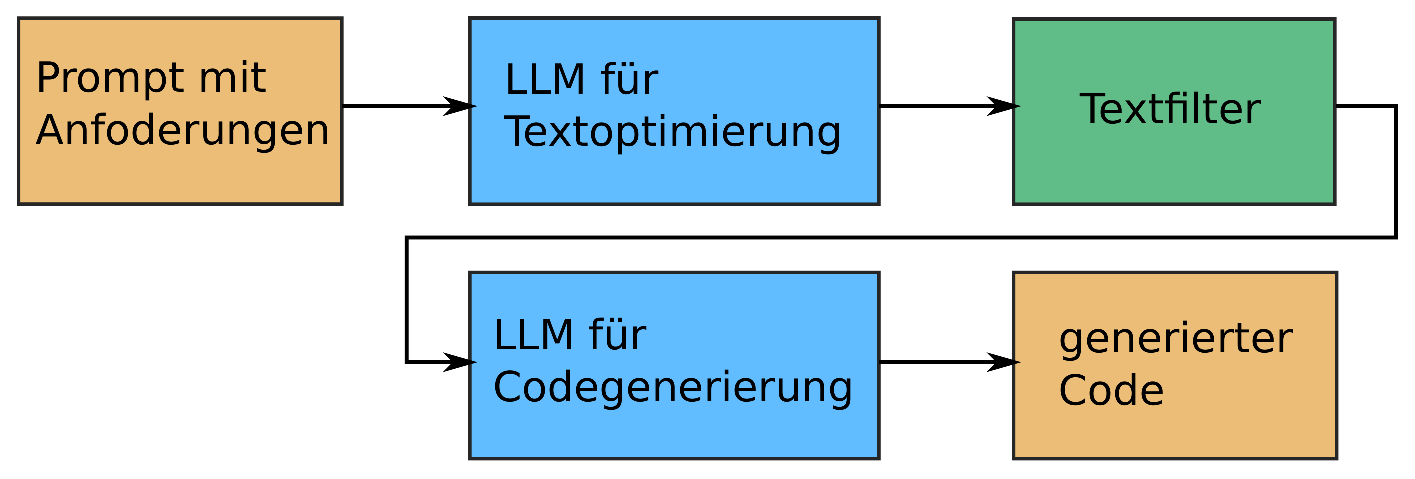
\includegraphics[width=0.8\textwidth]{content/chapter_implementation/images/orchestrierung_llms.eps}
%	\centering
%	\caption{Orchestrierte LLM's für die Codegenerierung}
%	\label{img:orchestration_llms}
%\end{figure}

%\section{Online Modelle}
%Text.

\subsection{Ergebnisse generieren}
Nachdem die Modelle bereitstehen, erfolgt das Generieren der Ergebnisse für jedes einzelne Modell. Mit Prompts, die aus den Proben des HumanEval-XL Benchmark bestehen, werden die Modelle mehrmals hintereinander abgefragt. Die vollständig generierten Antworten der Modelle werden, für eine spätere Auswertung und Nachvollziehbarkeit im \textit{JSONL}-Dateiformat gespeichert. Für jedes Problem erfolgen fünf Abfragen an jedes Modell. Welche Modelle für die Generierung verwendet wurden, ist in Kapitel \ref{subsec:llm_selection} nachzulesen. Alle Modelle wurde von Ollama-Framework bereitgestellt. Das Listing \ref{lst:python_generation_code} zeigt eine einfache Eingabeaufforderung, die an ein Modell gesandt wird.\vspace{0.2cm}

\begin{lstlisting}[
	language=Python,
	caption={Interaktion in Python mit Ollamaserver},
	label=lst:python_generation_code
]
from langchain_ollama.llms import OllamaLLM
from langchain.prompts import PromptTemplate

sample = read_sample_by(task_id=task_id)

model: OllamaLLM
answers: list = []
template = PromptTemplate(
    input_variables=["prompt"],
    template="{prompt}"
)
prompt = template.invoke({"user_prompt": sample.get("prompt")})

for index in range(0, 5):
    answers.append(model.invoke(prompt))

write_result(sample=sample.get("task_id"), answers=answers)
\end{lstlisting}

Nachdem die Proben in Zeile vier vom HumanEval-XL Benchmark eingelesen sind, wird in Zeile sechs bis zwölf das Modell und das Prompttemplate initialisiert. Um die Information \texttt{sample.get("prompt")} aus den Proben zu lesen, wird hier auf den Aufbau der Proben hingewiesen der in Kapitel \ref{subsec:structor_of_humaneval_xl} beschrieben wurde. Anschließend wird das Modell fünfmal abgefragt, hieraus lassen sich später, nach der \texttt{pass@k}-Methode, mit \texttt{k=\{0,...,5\}}, die Modelle evaluieren. Zum Schluss werden die Ergebnisse wie in Zeile siebzehn gezeigt, in JSONL-Dateien abgespeichert.

%---------------------------------------------------------------------------------------------------


\section{Optimierung der Antworten durch Änderung des Frameworks}
Wie das \texttt{langchain} Framework basiert das \texttt{DSPy} ebenfalls auf Python und eignet sich für die Abfrage lokale Ollama Modelle. Somit kann der vorhandene Ollama-Server genutzt werden.
Das Listing \ref{lst:python_generation_code_with_dspy} zeigt die einfache Initialisierung einer Interaktion mit einem lokalen Ollama Models mithilfe der \texttt{DSPy} Bibliothek.\vspace{0.2cm}

\begin{lstlisting}[
	language=Python,
	caption={Interaktion in Python mit Ollamaserver},
	label=lst:python_generation_code_with_dspy
]
import dspy

class BasicProgramming(dspy.Signature):
    question = dspy.InputField(desc="Eine Frage zu PHP Programmierung")
    answer = dspy.OutputField(desc="Generiere Programmcode")

model: dspy.LM = dspy.LM(
    api_base="http://192.168.1.56:11434", # required
    model="ollama_chat/deepseek-r1:32b", # required
    api_key="", # required
    temperature=0.2, # optinal
    cache=False, # optinal
    cache_in_memory=False, # optinal
)

dspy.configure(lm=model)
model(messages=[
    {
        "role": "user",
        "content": "Du bist erfahrener PHP Entwickler",
    }
])

chain = dspy.ChainOfThought(BasicProgramming)
\end{lstlisting}

Der Code zeigt Nach dem Bibliotheksimport wird die Signatur für die Abfrage erstellt. Hier wird die Interaktion mit dem Modell definiert. Es wird die erwartete Eingabe (\texttt{question}) und Ausgabe (\texttt{answer}) festgelegt. Die \texttt{desc}-Parameter im \texttt{InputField} und \texttt{OutputField} dienen lediglich für eine Beschreibung der Felder und haben keinen Einfluss auf den generierten Code.\vspace{0.2cm}

Im Anschluss wird das Lokale Modell mit erforderlichen und optionalen Parametern konfiguriert. Die Parameter \texttt{api\_base}, \texttt{model} und \texttt{api\_key} sind erforderlich. Wobei der Wert für \texttt{key} leer bleibt, solang der Ollama-Server keine Keys für die Anmeldung verwendet. Der Zusatz \texttt{ollama\_chat} veranlasst das Modell-Objekt nach einem Ollama-Server unter der, in \texttt{api\_base} angegebenen IP zu suchen. Mit einer \texttt{temperature}-Angabe von \texttt{0.2} wird das Modell zu einer deterministischen Antwort geleitet. Hier ist eine hohe Kreativität nicht gewünscht. Werden die optionalen Parameter \texttt{cache} und \texttt{cache\_in\_memory} nicht gesetzt, so wird ein Cache eingesetzt, was dazu führt, dass die Abfrage nur einmal in die LLM leitet und die Antwort in einem Cache abgelegt wird. Bei allen weiteren Anfragen würde diese Antwort wiederholt zurückliefert. Das würde bedeuten, das immer nur der $pass@k$ für $k=1$ erstellt werden könnte. Um dies zu verhindern, müssen beide Parameter den Wert \texttt{False} erhalten.\vspace{0.2cm}

Nachdem das Modell konfiguriert ist, wird in Zeile 16 DSPy mit dem Modell \texttt{model} konfiguriert und definiert somit deren Verwendung. Ab der Zeile 17 wird dann die Systemnachricht initialisiert. Diese Systemnachricht wird als erste Nachricht an die LLMs gesendet und legt dadurch den Kontext fest.\vspace{0.2cm}

Die letzte Zeile des Listings \ref{lst:python_generation_code_with_dspy} zeigt die Erstellung einer \texttt{ChainOfThought} Instanz mit der zuvor erstellten Signatur.


\subsection{Ergebnisse generieren}
\begin{tcolorbox}[
	enhanced,
	colback=red!5!white,
	colframe=red!75!black!50,
	title= Mein roter Faden
	]
	Mögliche Optimierungsstrategien
	\begin{itemize}
		\item mit dem Model Programming (DSPY) Ansatz: Python Bibliothek vorhanden \href{https://pypi.org/project/dspy/}{pypi.org | DSPy}.
	\end{itemize}
\end{tcolorbox}

%---------------------------------------------------------------------------------------------------


%\subsection{Auswertung der Modellantworten}
\section{Benchmark Codeevaluation}\label{sec:benchmark_evaluation}
Die Analyse der generierten Antworten muss für jedes Modell individuell angepasst werden, da die erzeugten Codefragmente zwischen den Modellen variieren. Insbesondere unterscheiden sich die Formate, in denen die Codesnippets generiert werden, beispielsweise durch \texttt{```php} oder \texttt{```php \textbackslash n <?php}. Dementsprechend erfordert die Extraktion des relevanten Codes aus den Modellantworten eine flexible Methode, die an das jeweilige Ausgabeformat der Modelle angepasst wird. Ein exemplarischer Lösungsansatz zur Extraktion des generierten Codes ist in Listing \ref{lst:code_extraction} dargestellt.\vspace{0.2cm}

\begin{lstlisting}[
	language=Python,
	caption={Codesnippet zur Extrahierung des Codes aus der LLM Antwort},
	label=lst:code_extraction
]
def get_generatet_code(code=code):
    if len(code.split("```php")) > 1: # find start
        code = code.split("```php")[1]
        code = code.split("```")[0]

    if code.startswith("<?php"): # find start
        code = code.split("<?php")[1]
        code = code.split("?>")[0]

    if len(code.split(r"\n}\n")) > 0: # find end
        code = code.split(r"\n}\n")[0] + "\n}\n"

    return code
\end{lstlisting}

Um den generierten Code zu evaluieren, wird dieser zusammen mit dem Test, der jeweiligen Probe aus dem Benchmark zusammengeführt. Das Ergebnis ist ein ausführbarer Code, der die geforderte Methode enthält. Mittels Python wird der Code getestet, ob der dieser ausführbar ist. Entsteht bei der Ausführung ein Laufzeitfehler erfolgt der Abbruch des Tests. Dieser kann ausgelöst werden durch eine nicht korrekte Syntax, einer Endlosschleife oder wenn die geforderte Methode nicht generiert wurde. All diese Ereignisse führen dazu, das die Probe als nicht bestanden gilt. Das Listing \ref{lst:php_interpreter_in_python} zeigt den Ausschnitt im Code zur Ausführung des PHP Interpreters in Python.\vspace{0.2cm}

\begin{lstlisting}[
language=Python,
caption={Codesnippet zur Ausführung des PHP Interpreters},
label=lst:php_interpreter_in_python
]
import subprocess

def test_answer(task_id, repetition):
    # read generated code
    answer = read_answer(task_id=task_id, repetition=repetition)
    answer = get_generatet_code(code=answer)

    # read test in HumanEval-XL
    test = read_sample(task_id=task_id).get("test")

    try:
        result = subprocess.run(
            ["php", "-r", f"{test}{answer}"],
            capture_output=True,
            text=True,
            check=False,
            timeout=5,
        )
    except subprocess.TimeoutExpired:
        return False

    if result.stderr.strip() == "":
        return True

    return False
\end{lstlisting}

Nachdem eine von fünf Antworten des Modells und der Test aus dem Benchmark vorliegen, erfolgt die Prüfung des generierten Codes. Diese wird im Listing \ref{lst:php_interpreter_in_python} ab Zeile zwölf gezeigt. Die Funktion liefert \texttt{True} zurück, wenn es keine Fehler im Test gab, sonst immer \texttt{False}. Das Exception-Handling ab Zeile 19 wird aufgerufen, wenn die PHP Ausführung in einer Schleife hängt. Hier wird ein \texttt{Timeout} abgefangen und somit gibt der Test als nicht bestanden. Aus den erhaltenen Ergebnissen, der Proben eines Tasks, berechnet die \texttt{pass@k} Methode, die \glqq Wahrscheinlichkeit das in \texttt{k}-Proben, eine korrekte Probe ist\grqq \, hinsichtlich Codegenerierung. Anschließend wird der Durchschnitt für die Zuverlässigkeit des Modells errechnet.\vspace{0.2cm}

\textbf{Umsetzung der pass@k Metric}\vspace{0.2cm}

Nach Abschluss der Tests werden die Ergebnisse mithilfe der \textit{pass@k}-Methode analysiert. In Python steht hierfür, die Bibliothek \textit{pass\_at\_k} zur Verfügung. Das Listing \ref{lst:custom_pass_at_k} zeigt die Implementierung der Methode gemäß Gleichung \ref{equ:pass_qt_k_complex} in Kapitel \ref{subsec:pass_at_k}, wie sie auch in der Python-Bibliothek verwendet wird.  


\begin{lstlisting}[
	language=Python,
	label=lst:custom_pass_at_k,
	caption={Berechnung der pass@k Metrik in Python}
]
def custom_pass_at_k(n: int, c: int, k: int) -> float:
    """
    :param n (int): numbers of total samples.
    :param c (int): number of currect samples.
    :param k (int): number of consider samples.
    """
    if n - c < k:
        return 1.0
    return 1.0 - np.prod(1.0 - k / np.arange(n - c + 1, n + 1))
\end{lstlisting}

%Die \textit{pass@k}-Methode dient zur Berechnung der Wahrscheinlichkeit, dass in $k$ Abfragen mindestens eine korrekte Lösung enthalten ist. Dazu
Die Methode erwartet drei Parameter. Der Parameter $n$ bezeichnet die Gesamtanzahl der Abfragen pro Probe. Der Parameter $c$ gibt die Anzahl der korrekten Abfragen innerhalb einer Probe an. Schließlich legt der Parameter $k$ fest, wie viele der besten Abfragen für die Bewertung berücksichtigt werden. Alle drei Parameter sind ganzzahlig (\texttt{Integer}), während das Ergebnis als Gleitkommazahl (\texttt{Float}) zurückgegeben wird.  

In dieser Arbeit werden die Werte $k=1$ und $k=5$ für die Evaluierung herangezogen. Nachdem jede Probe des HumanEval-XL-Benchmarks einzeln bewertet wurde, wird eine aggregierte Bewertung für das gesamte Modell ermittelt. Diese Berechnung erfolgt gemäß Gleichung \ref{equ:probability_of_success_per_model} in Kapitel \ref{subsec:pass_at_k}.  

% --- More Tests -----------------------------------------------------------------------------------


%\section{Codeevaluation mit Frameworks}
%Neben der bekannten Evaluationsmethode mit dem HumanEval Benchmark, wird hier eine weitere Testmethodik überprüft, die mit verschiedenen Validierungstools der jeweiligen Programmiersprache ausgeführt wird. Für die Erstellung der Abfragen wird das Python-Skript verwendet, was schon im Kapitel \ref{sec:benchmark_evaluation} vorgestellt wurde.

%\subsection{PHP Codeevaluation}
%Der Test wird bei den erweiterten Problemen durchgeführt und beginnt mit den Unit-Tests die mit \textit{PHPUnit} durchgeführt werden. Im Anschluss wird \textit{PHPMetrics} ausgeführt. Hierbei wird geprüft, ob die Codekomplexität und Wartbarkeit überprüft. Die Ausführung der Tests wird mithilfe eines Python-Skripts durchgeführt. Es wird eine PHP Datei erstellt, die mit den Frameworks geprüft wird.

%\subsection{JavaScript Codeevaluation}
%Text.

%\section{Online Modelle}
% Eigenen KI Server \href{https://www.computerweekly.com/de/ratgeber/Einen-KI-Server-mit-Ollama-und-Open-WebUI-einrichte}{Computer Weekly}
% Orchestrierung mit Python \href{https://pypi.org/project/multillm/}{multillm-Projekt}
% LangChain Library \href{https://python.langchain.com/api_reference/ollama/chat_models/langchain_ollama.chat_models.ChatOllama.html}{Example}
% \href{https://pypi.org/project/langchain-ollama/}{Python lib langchain-ollama}
% YouTube \href{https://www.youtube.com/@AICodeKing}{AICodeKing}

\chapter{Evaluation}\label{chap:evaluation}
Die Evaluation der Ergebnisse erfolgt im ersten Schritt anhand des HumanEval-XL Benchmarks. Dieser Benchmark wird in \cite{peng-2024} vorgestellt und erweitert den HumanEval \cite{chen-2021}. Der HumanEval-Benchmark evaluiert nur Python während der HumanEval-XL weitere Programmiersprachen und in verschiedenen Landessprachen unterstützt, darunter auch die deutsche Sprache. Neben Python sind auch Prompts für PHP und JavaScript enthalten, welche für die Webentwicklung wichtig sind. Die Datensätze des HumanEval-XL sind unter \href{https://github.com/FloatAI/humaneval-xl}{https://github.com/FloatAI/humaneval-xl} einsehbar und bestehen jeweils aus 80 Tests. Für jedes Problem werden zehn Lösungsvorschläge generiert, die im Anschluss auf die Aspekte der Syntaktik und Semantik evaluiert werden.\vspace{0.2cm}

Diese Tests fordern LLM's auf kleine Problem zu lösen. Aus diesem Grund werden weitere Tests erstellt mit umfangreicheren Anforderungen aus dem Bereich der Webentwicklung. Zu jedem Problem wird eine Musterlösung und ein Unittest erstellt. Der Aufbau für diese Bereitstellung orientiert sich an dem Format aus dem HunamEval-Benchmark.\vspace{0.2cm}

\begin{tcolorbox}[
	enhanced,
	colback=red!5!white,
	colframe=red!75!black!50,
	title= Mein roter Faden
	]
	Der nachfolgende Absatz wird sich noch mal ändern.  Je nachdem wie Aufwendig eine automatisierte Prüfung umsetzbar ist bzw. sich überhaupt automatisieren lässt.\vspace{0.2cm}
	
	Evtl. manuelle Auswertung von Stichproben.
\end{tcolorbox}

Des Weiteren ist die Bewertung der Coding-Standards der jeweiligen Programmiersprache vorgesehen. Für die Prüfung der Standards wird ein SonarQube-Server verwendet, der sowohl PHP als JavaScript unterstützt. Ebenfalls wird die Qualität des Codes evaluiert. Das Augenmerk liegt auf die Lesbarkeit, Effizienz und Wartbarkeit des generierten Codes.\vspace{0.2cm}

%Optional werden einige Tests von zusätzlichen Tools validiert, beispielsweise bei der Validierung von PHP Files sind es Tools wie phpunit\footnote{phpunit steht unter \href{https://github.com/sebastianbergmann/phpunit}{https://github.com/sebastianbergmann/phpunit} zum Download bereit.} und Code\_Sniffer\footnote{Code\_Sniffer steht unter \href{https://github.com/squizlabs/PHP_CodeSniffer}{https://github.com/squizlabs/PHP\_CodeSniffer} zum Download zur Verfügung.} für die Validierung von JavaScript findet das Framework Jasmin\footnote{\href{https://jasmine.github.io/}{https://jasmine.github.io}.} Anwendung.\vspace{0.2cm}


\section{Bewertung der Modelle}
Für die Bewertung wird das Vorgehen gewählt, welches in \cite{chen-2021} und \cite{peng-2024} beschrieben ist. Die Tests werden exemplarisch, mit den für die Webentwicklung relevanten Sprachen PHP und JavaScript durchgeführt. Die Evaluierung der Modelle wird auf den Ebenen \glqq einfache Fragen\grqq \ und \glqq komplexe Aufgaben\grqq \ erfolgen. Die \glqq einfachen Fragen\grqq \ werden bereits durch den zuvor genannten Benchmarks abgedeckt, sodass der entwickelte Fragenkatalog sich auf die Ebenen mit den \glqq komplexen Aufgaben\grqq \ konzentriert.\vspace{0.2cm}

Aus Ergebnisse der Tests, wird mithilfe der $pass@k$-Metrik, die Zuverlässigkeit der jeweiligen Modelle berechnet. Dieser Wert gibt an, mit welcher Wahrscheinlichkeit mindestens eine richtige Lösung unter $k$ ausgewählten Vorschlägen vorhanden ist. Die Formel \ref{equ:pass_qt_k} zeigt die Berechnung der $pass@k$-Metrik.

\begin{equation}\label{equ:pass_qt_k}
	\text{pass@k} = 1 - \frac{\prod_{i=0}^{n-k} (n - i - c)}{\prod_{i=0}^{n-k} (n - i)}
\end{equation}

Dabei ist $n$ die Gesamtanzahl der Versuche, $c$ die Anzahl der korrekten Lösungen unter den $n$ Versuchen und $k$ gibt die Anzahl der Lösungen an die betrachtet wurden.

%--- Optimierung --------------------------------------------------------------------------------


\section{Optimierung der Ergebnisse}
Ein Ansatz zur Optimierung der Ergebnisse ist, ...

% https://ki-techlab.de/ki-news/evaluierung-grosser-sprachmodelle-ein-technischer-leitfaden/

%\begin{tcolorbox}[
%	enhanced,
%	colback=BhtColorYellow!5!white,
%	colframe=BhtColorYellow!75!black,
%	title= HTML Startseite
%	]
%	Text in der Box
%\end{tcolorbox}

%\begin{tcolorbox}[
%	enhanced,
%	colback=BhtGrey!5!white,
%	colframe=BhtGrey!75!black!50,
%	title= ChatGPT 3.5
%	]
% Text in der Box
%\end{tcolorbox}


\chapter{Lessons Learned}\label{chap:lessons_learned}
\begin{tcolorbox}[
	enhanced,
	colback=red!5!white,
	colframe=red!75!black!50,
	title= Mein roter Faden
	]
Dieses Kapitel wird die positiven und negativen Erfahrungen der Kapitel Implementierung und Evaluation auffassen. Die weiteren Kapitel bauen auf die hier gewonnenen Erkenntnisse auf.
\end{tcolorbox}


\section{Erweiterte Codeevaluation}
Bei den vordefinierten Prüfungen der HumanEval Benchmarks, wird geprüft, ob der Code lauffähig ist, nicht aber die Codestruktur oder Kommentare. Ein Problem bei der Nutzung des von der LLM generiertem Code ist, dass Entwickler diesen einfach kopieren und in ihre Programme implementieren. Es wird also nur die Funktionalität des Codes geprüft, nicht aber Strukturen und Kommentare um die Lesbarkeit und Verständlichkeit zu erhöhen. Dieses Vorgehen mag zu schnellen Erfolgen in der Programmentwicklung führen, wird aber beim Refactoring oder Fehlersuche erhebliche Defizite mit sich bringen.\vspace{0.2cm}

Aus diesem Grund sollte der erstellte Code nicht nur auf die Funktionalität geprüft werden. Dafür sollten weitere Test-Frameworks der jeweiligen Programmiersprache zur Anwendung kommen. Es gibt mehrere Frameworks zur Prüfung der Codequalität unter PHP. Zwei bekannte Frameworks die auch in dieser Arbeit Anwendung finden, sind die Frameworks \texttt{phpunit} und \texttt{phpmetrics}. Mit ihnen wird der, durch die LLMs generierten Codes geprüft.\vspace{0.2cm}

Um PHPUnit und PHPMetrics für die Evaluierung zu verwenden, müssen weitere Angaben und Einträge im Benchmark erfolgen. So muss ein PHP-Unittest enthalten sein, dieser kann den einfachen benutzerdefinierten Test ersetzen. Des Weiteren sind die Kriterien für die Metrik Messung, für jeden Test erforderlich. Die Kriterien können wie in Listing \ref{lst:phpmetric_criteria_example} dargestellt, aussehen.

\begin{lstlisting}[language=python,caption={Beispiel für Bewertungskriterien},label=lst:phpmetric_criteria_example]
	criteria = {
		"Lines of code": lambda x: int(x) > 12,
		"Logical lines of code by method": lambda x: float(x) > 7,
		"Lack of cohesion of methods": lambda x: float(x) > 3,
		"Average Cyclomatic complexity by class": lambda x: float(x) > 10,
		"Average Weighted method count by class": lambda x: float(x) > 20,
		"Average bugs by class": lambda x: float(x) > 0.1,
		"Critical": lambda x: int(x) > 0,
		"Error": lambda x: int(x) > 0,
		"Warning": lambda x: int(x) > 0,
		"Information": lambda x: int(x) > 0,
	}
\end{lstlisting}

Mit den erweiterten Tests werden die Benchmarks, um die folgenden Punkte erweitert.

\begin{myitemize}
	\item \textbf{unittest}: Unittests für die geforderte Funktion, unterschied zu den einfachen Tests
	\item \textbf{metrics}: Kriterien für den Metriktest
\end{myitemize}

\subsection{PHPUnit}
Eines der bekanntesten spezielles Framework für Unit-Tests in PHP, was als Industriestandard gilt. Mit diesem Framework können neben der Prüfung auf funktionsfähigen Code auch Randfälle betrachtet und Fehlerbehandlungen im Code getestet werden. Als Grundlage für die Auswahl des Tools wird auf Studie \cite{mohamad-2016} verwiesen.

\subsection{PHPMetrics}
Ein PHP Framework für die Codeanalyse, welches detaillierte Berichte über die Codequalität, Komplexität des Codes und über dessen Wartbarkeit erzeugt. PHPMetrics wird in verschiedenen Arbeiten eingesetzt, um die Codequalität zu ermitteln. So auch in \cite{anggrain-2016}, bei der verschiedene Open Source LMS verglichen werden.

\subsection{SonarQube}
Als letztes Tool soll SonarQube zur statischen Codeanalyse und Codeprüfung zum Einsatz kommen. Es werden verschiedene Programmiersprachen unterstützt, darunter auch PHP und JavaScript. In der Arbeit \cite{da-silva-simoes-2024} wird die Prüfung der Codequalität mit SonarQube, ChatGPT3.5 und ChatGPT4 vergleichen. Als Schlussfolgerung aus dem Ergebnis dieser Arbeit, wird auch hier die Codeanalyse durch eine LLM nicht erfolgen, sondern ebenfalls durch SonarQube.

%\subsection{ESLint}
%JavaScript Tool zur Syntaxfehler-Erkennung, Stil- und Codequalitätsprüfung. Mit diesem Tool kann reines JavaScript als auch Node.js überprüfen. https://arxiv.org/html/2402.14261v1


\chapter{Diskussion und Ausblick}\label{chap:discussion}
\begin{tcolorbox}[
	enhanced,
	colback=red!5!white,
	colframe=red!75!black!50,
	title= Mein roter Faden
	]
	Struktur des Kapitels
	
	\begin{enumerate}
		\item \textbf{Einleitung}: Eine kurze Einführung in die Diskussion und den Ausblick.
		\item \textbf{Zusammenfassung der Ergebnisse}: Eine kurze Übersicht über die wichtigsten Ergebnisse und in Relation mit den Forschungsfragen stellen.
		\item \textbf{Diskussion der Ergebnisse}: Eine Analyse und Interpretation der Ergebnisse. Vergleich mit Stand der Forschung und früherer Arbeiten.
		\item \textbf{Grenzen und Einschränkungen}: Eine Diskussion der Limitationen der Studie. Z.B. begrenzte Datenbasis, Grenzen der eingesetzter Tools und Technik.
		\item \textbf{Impulse für zukünftige Forschung}: Vorschläge für weitere Studien. Verbesserungsmöglichkeiten der Methoden usw. und Zukunft des Forschungsfeldes und evtl. Trends.
		\item \textbf{Praktische Anwendung}: Eine Diskussion der möglichen Anwendungen der Ergebnisse. In welchen Unternehmen und welche realen Anwendungen können die Ergebnisse eingesetzt werden.
	\end{enumerate}
\end{tcolorbox}

Wie in \cite{hartenstein_2024} beschrieben,
\section{Thesen}
% 3. These: Optimierung ohne Modellanpassung, nur Prompt Engineering
Die Erkenntnisse aus den Experimenten dieser Arbeit bestätigen die aufgestellte dritte These (T3) aus Kapitel \ref{sec:goals_of_the_work}. Eine Optimierung der Eingabeaufforderungen für die Webanwendungsentwicklung lässt sich ohne Änderung der Modellparameter erreichen und bewirken eine signifikante Verbesserung der Ergebnisse. Die Modelle wurden bereits mit Programmiersprachen, die für Webanwendungsentwicklung essenziell sind, wie beispielsweise PHP, trainiert und diese Daten, in Form von Programmcode sind in den Modellen abrufbar. Entscheidend hierbei ist die Art und Weise wie die Gestaltung der Eingabeaufforderungen umgesetzt wird. Diese Optimierung erfolgt durch das \texttt{DSPy} Framework für die meisten Modelle automatisch.\vspace{0.2cm}

Dennoch hat das \texttt{DSPy} Framework, auf einige Modelle eine negative Auswirkung. Der generierte Code schnitt in der Evaluation mit den HumanEval-XL Proben schlechter ab. Das legt die Annahme nahe das  

Aus diesem Grund sollte in diesen Fällen weitere Frameworks, wie beispielsweise \textit{AdalFlow} oder \textit{LamaIndex} für die Optimierung in Betracht gezogen werden.\vspace{0.2cm}

% 2. These: Benckmarks sind ungeeignet
Diese Erkenntnis lassen den Schluss zu, dass die zweite These (T2) aus Kapitel \ref{sec:goals_of_the_work} bewiesen wurde. Ein einzelner Benchmark hat nicht ausreichend Aussagekraft, um eine LLMs hinreichend zu bewerten. Diese Benchmark eignen sich dafür einen ersten Eindruck von den Modellen zu erhalten. Wie auch in \cite{zhang-2024} wird die Auffassung vertreten, dass diese Probe grundlegende Codeproblematiken testen, die nicht mit den realen Bedingungen übereinstimmen. In dem Onlineartikel \cite{albrecht-2023} heißt es \glqq \textit{...liefert Code, der zwar nicht immer direkt nutzbar ist, nach einer Überarbeitung aber schon recht überzeugend läuft.}\grqq \ was darauf hindeutet, dass Programmierer andere Anforderungen an LLMs stellen, die zurzeit mit Benchmarks nicht abgedeckt werden können.\vspace{0.2cm}

% 1. These: LLMs effizientere Webanwendungsentwicklung. Wichtig ist die Evaluierung
In den letzten Jahren hat generative KI auch die Arbeit der Entwickler stark beeinflusst. So ist in \cite{focus-online-2025} die Rede von einem Programmierer, der seine Aufgabe ab brach, \glqq \textit{weil er keinen Zugang zu seinem virtuellen Assistenten hatte. ''Ich kann einfach nicht mehr ohne die Hilfe der KI programmieren''}\grqq \ so der Entwickler. So werden KI Anwendungen bei Entwicklern immer beliebter und das gilt auch für den Bereich der Webanwendungsentwicklung. Dabei verwenden viele Entwickler KI Modellen von US Amerikanischen Unternehmen wie Athropic, Google oder OpenAI

\section{Impulse für zukünftige Forschungen}
Ein interessantes Feld für die Forschung ist die Nutzung generativer KI und welche Auswirkungen dies auf das menschliche Denken und Handeln hat. In der Studie \cite{chiriatti-2024} wird von einem System 0 gesprochen, welches neben den bekannten 
\begin{enumerate}
	\item System 1: schnelles,intuitives und automatisches Denken
	\item System 2: langsameres, analytisches und reflektierteres Denken
\end{enumerate}

eingeführt wird. Hierbei handelt es sich um ein Denken, welches die KI für den Menschen übernimmt. Entscheidungen und Daten werden durch die KI übernommen. Ein externes System, ähnlich wie eine USB-Festplatte eines PCs.\vspace{0.2cm}

Inwieweit können auch \textit{Small Language Models} für Programmieraufgaben eingesetzt werden. Könnte der enorme Energiebedarf und Ressourcen der LLMs durch SLMs ersetzt werden? Siehe 
\href{https://medium.com/@nageshmashette32/small-language-models-slms-305597c9edf2}{Small Language Models (SLMs)} oder \href{https://medium.com/version-1/small-but-powerful-a-deep-dive-into-small-language-models-slms-b793bdb002f2}{Small but Powerful: A Deep Dive into Small Language Models (SLMs)}. Eine weitere Forschung kann die Evaluation sein, ob Finetuned SLMs, wie Phi-2, Google Gemini Nano oder Metas Llama-2-13b bessere Ergebnisse liefern, als die LLMs.\vspace{0.2cm}

Ein weiteres Feld kann sich mit der Einführung einer KI in Firmen befassen und Fragen wie,

\begin{itemize}
	\item Wie können Entwickler bestmöglich vorbereitet werden, um die Einführung von KI reibungslos zu ermöglichen?
	\item Wie kann Datensicherheit und Datenqualität sichergestellt werden?
	\item Evaluierung von Kosten/Nutzen für die Einführung von KI in Softwareunternehmen.
\end{itemize}

evaluieren.


%\begin{tcolorbox}[
%	enhanced,
%	breakable,
%	colback=red!5!white,
%	colframe=red!75!black!50,
%	title= Mein roter Faden: noch was zum Testen
%	]
%	Ein Tool zur Orchestrierung von Multi-Agenten-Systemen \href{https://community.openai.com/t/introducing-swarm-js-node-js-implementation-of-openai-swarm/977510}{OpenAI Swarm}, gefunden auf \href{https://karrierewelt.golem.de/blogs/karriere-ratgeber/bot-belegschaft-mit-entlastungspotenzial-ki-agenten-fur-den-arbeitsalltag-in-der-testphase-1}{Golem | Karrierrewelt}.
%\end{tcolorbox}

\section{Praktische Anwendung}
Blaupause für Prompting \href{https://piamedia.com/wp-content/uploads/2024/09/PIAM_Whitepaper_LLM-Halluzinationen_DE.pdf}{Das Geheimnis hinter LLM-Halluzinationen} [S. 16 ff.] noch testen und evaluieren.

\href{https://arxiv.org/html/2501.16998v1}{Große Sprachmodelle zur Codegenerierung: Die Perspektive der Praktiker}

\subsection{Anwendung für Entwickler}
Zur Optimierung des generierten Codes kann auch die freie Wahl der Softwarekomponenten durch die LLMs betragen. Wie in \cite{chen-2021} beschrieben können Nutzer, anstatt in Suchmaschinen beispielsweise die Vorteilen und Nachteile von \texttt{PyTorch} und \texttt{Tensorflow} zu vergleichen, kann das die LLM übernehmen und als Prompt wird nur \texttt{\# import machine learning package} angegeben.\vspace{0.2cm}

Wie in [Quelle ist weg] beschrieben nimmt das Lesen von Programm zehn mal mehr Zeit in Anspruch, als Code zu schreiben. Diese Arbeit kann ebenfalls durch eine LLM übernommen werden.

\chapter{Fazit}\label{chap:conclusion}
Es gibt Modelle welche besonders für die Webanwendungsentwicklung sehr gute Ergebnisse, auch ohne Optimierung liefern. Dennoch sollte eine Optimierung der Eingabeaufforderungen in Betracht gezogen werden, da diese mit relativ wenig Aufwand umsetzbar ist. Der Einsatz von generativer KI wird in alles Bereichen der Programmierung neue Maßstäbe setzen und nachhaltig verändern. Dieser Prozess hat bereits begonnen und immer mehr Unternehmen befassen sich mit diesem Thema und investieren in den Ausbau dieser Technologie. Dies bedeutet, dass eine Transformation auf Unternehmensebene durchzuführen ist, welche die gesamten Prozesse der Codegenerierung umfasst, auch wenn diese Transformation zu Beginn höhere Kosten verursacht.\vspace{0.2cm}

Es wird festgestellt, dass durch die Evaluation mit Benchmarks eine relevante Kenngröße zur Ermittlung der optimalen LLM gemessen werden kann, obwohl durch die Benchmarks nicht alle Aspekte der Webanwendungsentwicklung abgedeckt werden können. Ebenfalls ist es wichtig, Kenntnisse über die Auswahl geeignete Methoden in Form von Frameworks oder die Wahl der Sprache zu kennen, um die geeignete LLM auszuwählen.\vspace{0.2cm}

Alle, in dieser Arbeit vorgeschlagenen Ansätze, können langfristig zu einer Kosteneinsparung beitragen, da sich der Ressourcenverbrauch reduzieren wird. Dies wird sich bei die Entwicklungszeit für Anwendungen, für die Fehlersuche und beim Implementieren von zusätzlichen Funktionen bemerkbar machen.
% Documents
% https://arxiv.org/abs/2109.04738: On the validity of pre-trained transformers for natural language processing in the software engineering domain
% https://arxiv.org/abs/2204.03214: Transformer-Based Language Models for Software Vulnerability Detection
%
% Tutorials
% https://towardsdatascience.com/building-a-python-code-generator-4b476eec5804

	\newpage
	\backmatter

\addcontentsline{toc}{chapter}{Literatur}
\printbibliography

%\addcontentsline{toc}{chapter}{Glossar}
%\printglossary

\renewcommand\thesection{\Alph{section}}
\renewcommand\thesubsection{\thesection.\arabic{subsection}}
\chapter{Anhang}
\section{Installationshinweise}
\subsection{Python}
Da in dieser Arbeit Python verwendet wird, sollte zu den grundlegenden Paketen, für die Arbeit mit großen Sprachmodellen folgende Zusatzpakete installiert sein.

\begin{verbatim}
	pip3 install langchain
	pip3 install ollama
	pip3 install transformer
\end{verbatim}

Im Weiteren wird kein Hinweis auf verwendete Pakete gegeben. Diese sind evtl. den Fehlermeldungen während und nach der Programmausführung zu entnehmen.

\subsection{Installation und Konfiguration von Ollama}\label{sec:install_config_ollama_local}
Für die Installation von Ollama wird bei Linux folgendes Skript ausgeführt,

\begin{verbatim}
	curl -fsSL https://ollama.com/install.sh | sh
\end{verbatim}

Ollama kann in seiner Konfiguration angepasst werden, im Folgenden wurde der Pfad zur den Modellen geändert und die Erreichbarkeit von Ollama über Netzwerk eingestellt. Dazu wird die Datei  \texttt{/etc/systemd/system/ollama.service} angepasst und der korrekte Host und IP-Adresse gesetzt.

\begin{lstlisting}[language=diff,caption={Ollama Hostanpasssng für Netzwerkbetrieb}]
	diff --git a/ollama.service b/ollama.service
	--- a/ollama.service
	+++ b/ollama.service
	@@ -10,3 +10,4 @@
	RestartSec=3
	Environment="PATH=/usr/local/bin:/usr/bin"
	-   
	+   Environment="OLLAMA_HOST=0.0.0.0"
	+   Environment="OLLAMA_MODELS=/home/ai/models"
	+   
\end{lstlisting}

Nach der Installation kann die Funktionsfähigkeit geprüft werden, der folgenden Beispielaufruf lädt ein Modell von Ollama und startet dieses.

\begin{verbatim}
	ollama run deepseek-coder-v2:16b
\end{verbatim}

Im Anschluss kann über die Konsole mit dem Modell interagiert werden.

%---------------------------------------------------------------------------------------------------


\subsection{Open WebUI Installationshinweise}\label{sec:open_webui}
Hier wird Open WebUI als docker Container verwendet, es ist also erforderlich vorher docker zu installieren. Die Installation von Open WebUI, unter Debian kann mit folgendem Skript erfolgen. 

%\begin{verbatim}
\begin{lstlisting}[language=bash,caption={Open WebUI installieren}]
# Pull Open WebUI container.
docker pull ghcr.io/open-webui/open-webui:main

# Run container.
docker run -d --network=host -v open-webui:/app/backend/data \
-e OLLAMA_BASE_URL=http://127.0.0.1:11434 --name open-webui \
--restart always ghcr.io/open-webui/open-webui:main
\end{lstlisting}
%\end{verbatim}

Der Aufruf der UI, kann mittel Browser erfolgen. Hier wird die IP und der Port 8080 angegeben. Beispiel \texttt{http://192.168.2.45:8080}.

%---------------------------------------------------------------------------------------------------

\newpage
\section{Download der Hugging Face Modelle}\label{sec:hugging_face_models}
Ein Hugging Face Modell kann, heruntergeladen werden. Soll das Modell auch nach dem Löschen des lokalen \texttt{huggingface}-Caches zur Verfügung stehen, sollte das Modell separat abgespeichert werden. Für den Download und speichern der Modelle kommt das Python-Skript, wie in Listing \ref{lst:download_hugging_face_model} gezeigt zur Anwendung. Hier ist zu erwähnen, dass ausreichend RAM zur Verfügung stehen muss, um die Modelle zu speichern. Mit diesem Script kann ein Modell an einem angegebenen Pfad abgespeichert werden und ist nach dem Cache löschen immer noch lokal vorhanden.

\lstinputlisting[
	language=python,
	caption={Laden der Modelle von Hugging Face und lokal speichern},
	label=lst:download_hugging_face_model
]{codes/src/download/huggingface_model.py}

\newpage
\section{Abfragen lokaler Modelle}
Um die Modelle abzufragen, kommt der Code, welcher in Listing \ref{lst:call_ollama_model} zu sehen ist, zum Einsatz.

\lstinputlisting[
	language=python,
	caption={Abfragen der Ollama Modelle},
	label=lst:call_ollama_model
]{codes/src/execute/execute_ollama.py}

\newpage
\section{Abfrage cloudbasierter Modelle}

\lstinputlisting[
	language=python,
	caption={Ausführen der Prompts für Gemini Modelle.},
	label=lst:execution_gemini_models
]{codes/src/execute/execute_google_gemini.py}

\lstinputlisting[
	language=python,
	caption={Ausführen der Prompts für OpenAI Modelle.},
	label=lst:execution_openai_models
]{codes/src/execute/execute_openai_gpt.py}


\subsection{Evaluation der Antworten von den Modellen}
Das Listing \ref{lst:evaluation_search_generated_code} zeigt beispielhaft eine Suche nach Codezeilen in einer Antwort eines Modells. Die Methode \texttt{search\_generated\_code} muss auf jedes Modell angepasst sein.

\begin{lstlisting}[
	language=python,
	caption={Evaluation der Modellantworten: Suche nach Codeausschnitten},
	label=lst:evaluation_search_generated_code
]
def search_generated_code(content: str) -> str:
    """
    Search the generated code in string, it is one line of file.
    :param content (str): Answer from LLM.
    :returns str: Generated code.
    """
    for index in [i for i in range(0, 10)]:
        if content.startswith('{"result_' + str(index) + '":"'):
            generated_code: str = content.split(
                '{"result_' + str(index) + '":"')[1]
            generated_code = generated_code[:-2]
            generated_code = generated_code.strip()

        if len(generated_code.split("```php")) > 1:
            generated_code = generated_code.split("```php")[1]
            generated_code = generated_code.split("```")[0]

        if generated_code.startswith("<?php"):
            generated_code = generated_code.split("<?php")[1]
            generated_code = generated_code.split("?>")[0]

        if len(generated_code.split(r"\n}\n")) > 0:
            generated_code = generated_code.split(r"\n}\n")[0] + "\n}\n"

        return generated_code
    return ""
\end{lstlisting}


\newpage
\section{Methodenerkennung unter PHP}
Mit den folgenden Skripten wird gezeigt das es möglich ist PHP Funktionen welche durch LLMs erzeugt wurden zu scannen und beispielsweise deren Namen in Tests verwenden zu können. Das Listing \ref{lst:php_code_functions} zeigt ein Skript, das beispielhaft verschiedene Funktionen implementiert die durch das Skript im Listing \ref{lst:php_code_scan_functions} zur Laufzeit erkannt werden.\vspace{0.2cm}

\begin{lstlisting}[
	language=php,
	caption={PHP Skript welches verschiedene Funktionen imlementiert},
	label=lst:php_code_functions
]
<?php
// @file: methods.php

function fibfib_rekursiv($n) {}

function fibfib_iterativ($n) {}

function fib($x, $y) {}

function fibfib($n) {}

\end{lstlisting}

\begin{lstlisting}[
	language=php,
	caption={PHP Skript das Methoden zur Laufzeit erkennt},
	label=lst:php_code_scan_functions
]
<?php
// @file scan_methods.php

<?php

// include "method_names.php";
$filename = "method_names.php";
$code = file_get_contents($filename);
$tokens = token_get_all($code);

$all = [];
$search = "";
$func_name = False;
foreach ($tokens as $token) {
	if (
		gettype($token) == "array" &&
		count($token) > 1 &&
		trim($token[1]) != "" &&
		trim($token[1]) !="<?php"
	) {
		if ($token[1] == "function") {
			if (str_ends_with($search, ",")) {
				$search = substr($search, 0, strlen($search) - 1);
			}
			$search = $search . ")";
			if ($search  != ")") {
				$all[] = $search;
			}
			$search = $token[1] . " ";
			$func_name = True;
		} elseif ($func_name) {
			$func_name = False;
			$search = $search . $token[1] . "(";
		} else {
			$search = $search . $token[1] . ",";
		}
	}
}

if (str_ends_with($search, ",")) {
	$search = substr($search, 0, strlen($search) - 1);
}

$search = $search . ")";
$all[] = $search;

print_r($all);
\end{lstlisting}

Nach dem Ausführen des Skriptes wird die Ausgabe, welche in Listing \ref{bash_scan_function_result} zu sehen ist erzeugt.

\begin{lstlisting}[
	language=bash,
	caption={Erkannte PHP Methoden},
	label=lst:bash_scan_function_result
]
Array
(
    [0] => function fibfib_rekursiv($n)
    [1] => function fibfib_iterativ($n)
    [2] => function fib($x,$y)
    [3] => function fibfib($n)
)
\end{lstlisting}


%\section{Fragenkataloge}
Die Fragenkataloge enthalten Aufgaben welche an die großen Sprachmodelle gesendet und dessen Antwort evaluiert wurde. Die Struktur der Fragen ähnelt dem Benchmark aus \cite{peng-2024}.

\subsection{PHP}
Alle Fragen in diesem Katalog sind in der natürlichen Sprache Deutsch verfasst und als Programmiersprache in PHP.

\begin{tcolorbox}[
	enhanced,
	colback=white,
	coltitle=black,
	colbacktitle=white,
	title= php/f0 - JSON Informationen in einer MySQL speichern
	]
	\textbf{Ziel:}\\
	Hierbei wird die Fähigkeit geprüft, ob LLM die Konvertierung der JSON Daten in SQL Format korrekt erledigt wird, insbesondere das Datumsformat. Den Verbindungsaufbau zu einer Datenbank, sowie das erstellen und füllen von Tabellen. Ebenso wird ein Test erwartet, der den generierten Code testet.\\
	\textbf{Aufgabe:}\\
	Du bist ein PHP Entwickler und hast folgende Aufgabe:\\
	Erstelle einen Backendservice der Daten aus einem JSON String in einer SQL Datenbank speichert.\\
	Die Methode convAndSaveData, die die Aufgabe erfüllt, soll sich in der Klasse RestService befinden. Die Datenbankparameter sollen als Klassenattribute vorliegen und die Kommunikation mit der Datenbank in einer privaten Methode gekapselt werden. Die Daten sollen in den Tabellen ,,user'' und ,,address'' gespeichert werden. Die Felder in der Tabelle entsprechen denen aus dem JSON. Prüfe ob die Tabellen vorhanden sind, wenn nicht legt diese an. Verwende kein Framework wie Laravel oder Symfony, sondern nur PHP Funktionen.\\
	Die Daten im JSON haben folgendes Format:\\
	\texttt{\{''firstname'':  ''Max'', ''surname'': ''Musterman'',''birthday'': ''20.3.1990'',''address'': \{"street": ''Straße'',''streetnumber'': 3,''streetaddon'': ''A'',''postcode'': ''12345'',''town'': ''Berlin''\}\}}

	\textbf{Erwartetes Ergebnis:}\\
	Am Testende wurden in der MySQL Datenbank zwei Tabellen \glqq user\grqq \ und \glqq address\grqq \ angelegt, welche mit den Beispieldaten aus der Formatbeschreibung gefüllt wurden.
\end{tcolorbox}


\subsection{JavaScript}


\mainmatter
\chapter*{Anlagen}
%\addcontentsline{toc}{chapter}{Anlagen}
{\Huge Erklärung zur Verwendung von KI-Systemen}\vspace{0.5cm}

Ich erkläre, dass ich

\begin{myitemize}
	\item mich aktiv über die Leistungsfähigkeit und Beschränkungen der in meiner Arbeit eingesetzten KI-Systeme informiert habe;
	\item alle Inhalte aus wissenschaftlich anerkannten Quellen entnommen und entsprechend gekennzeichnet habe; alle Inhalte unter Anwendung wissenschaftlicher Methoden im Rahmen der vorliegenden Arbeit von mir selbst entwickelt wurden;
	\item mir bewusst bin, dass ich als Autor*in dieser Arbeit die Verantwortung für die in ihr gemachten Angaben und Aussagen trage.
\end{myitemize}

Bei der Erstellung der Arbeit habe ich die folgenden auf künstlicher Intelligenz (KI) basierten Systeme in der
im Folgenden dargestellten Weise benutzt:

\begin{longtable}[H]{{|p{0.23\linewidth}|p{0.20\linewidth}|p{0.49\linewidth}|}}
		\hline
	\textbf{Arbeitsschritt} & \textbf{Eingesetzte(s) KI-System(e)} & \textbf{Beschreibung der Verwendungsweise} \\
	\hline
	Generierung von Ideen und Konzeption der Arbeit & - - - - & - - - - \\
	\hline
	Literatursuche & - - - - & - - - - \\
	\hline
	Literaturanalyse & - - - - & - - - - \\
	\hline
	Literaturverwaltung und Zitationsmanagement & - - - - & - - - - \\
	\hline
	Auswahl der Methoden und Modelle & - - - - & - - - - \\
	\hline
	Datensammlung und -analyse & - - - - & - - - - \\
	\hline
	Generierung von Programmcodes & ChatGPT und Gemini & Erstellen grundlegender Anweisungen und Coderecherche für Python \\
	\hline
	Erstellung von Visualisierungen & - - - - & - - - - \\
	\hline
	Interpretation und Validierung & - - - - & - - - - \\
	\hline
	Strukturierung des Texts der Arbeit & ChatGPT & Generierung von Vorschlägen für den Aufbau der Kapitel \\
	\hline
	Formulierung des Texts der Arbeit & ChatGPT & Umformulieren von Absätzen, mit denen ich nicht zufrieden war \\
	\hline
	Übersetzung des Texts der Arbeit & DeepL & Übersetzung von Text für eigenen Code \\
	\hline
	Redigieren des Texts & ChatGPT und Duden Online & Korrektur von Rechtschreibfehlern und Grammatikfehlern und Umstrukturierung von Satzbau \\
	\hline
	Vorbereitung der Präsentation des Texts & - - - - & - - - - \\
	\hline
	Sonstiges & - - - - & - - - - \\
	\hline
\end{longtable}\vspace{2.0cm}

\underline{Temmen-Ringenwalde, \today} \hspace{1cm} \underline{, \hspace{6cm}}

\hspace{0.2cm} Ort, Datum \hspace{5.2cm} Unterschrift


\end{document}
